\chapter{Usporedba API-ja i ograničenja sustava}

\section{Usporedba aplikacijskih sučelja}

Za analizu i usporedbu API-ja odnosno demo aplikacija korištena je mobilna aplikacija \textit{nRF Connect} tvrtke \textit{Nordic Semiconductor}. Pomoću nje moguće je pretražiti i povezati se sa BLE uređajima, kao i komunicirati s njima. Aplikacijom se također mogu analizirati podaci koje uređaj šalje pri oglašavanju te čitati informacije o samim uređajima i uslugama koje nude. \cite{nrfapp}

Jedna od mogućnosti aplikacije je i prikaz RSSI (engl. \textit{Received Signal Strength Indicator}) grafa. To je pokazatelj jačine primljenog signala te služi za mjerenje snage u primljenom radio signalu. RSSI je glavni indikator o jačini signala u danoj točki prostora. RSSI je relativna mjera, stoga je na grafičkom prikazu os RSSI vrijednosti označena dBm skalom, koja je negativna. 

\begin{figure}[ht]
	\begin{minipage}[t]{0.4\textwidth}
		\includegraphics[width=\linewidth]{imgs/graph\_all}
		\label{fig:graph_all}
	\end{minipage}
	\hspace*{\fill}
	\begin{minipage}[t]{0.4\textwidth}
		\includegraphics[width=\linewidth]{imgs/graph\_all2}
		\label{fig:graph_all2}
	\end{minipage}
	\caption{Graf RSSI vrijednosti u ovisnosti o vremenu za \textit{Bluedroid} demo aplikacije}
\end{figure}

\section{Ograničenja razvojnog sustava}

Klasična Bluetooth tehnologija razvijena je kao bežični standard, što je omogućilo razvoj bežičnih i prenosivih uređaja. \textit{BT Classic} tehnologija koristi se za \textit{streaming} aplikacije, poput prijenosa audiozapisa i datoteka. Radi na istim frekvencijama kao i BLE, no ima veći broj RF kanala. Klasični Bluetooth ima veću propusnost podataka, čak do 2.1 Mbps, dok BLE propušta maksimalno 0.27 Mbps. Također ima veću brzinu prijenosa podataka, do 3 Mbps, u usporedbi sa BLE protokolom čija brzina doseže najviše 1 Mbps. Za razliku od BLE protokola čija je glavna odlika niska potrošnja,  zbog brze i nepredvidive komunikacije te složenih postupaka povezivanja \textit{BT Classic} troši znatno više energije i time brže troši bateriju uređaja na kojem se nalazi. Latencija prijenosa je čak 16 puta veća nego u BLE uređajima. Isto tako, podržava samo \textit{peer-to-peer} topologiju, odnosno 1:1, što znači da se istovremeno mogu povezati samo dva uređaja. Detaljnije razlike između verzija Bluetooth protokola nalaze se na slici \ref{fig:blevsbt}. \cite{blevsbt}

\begin{figure}[ht]
	\centering
	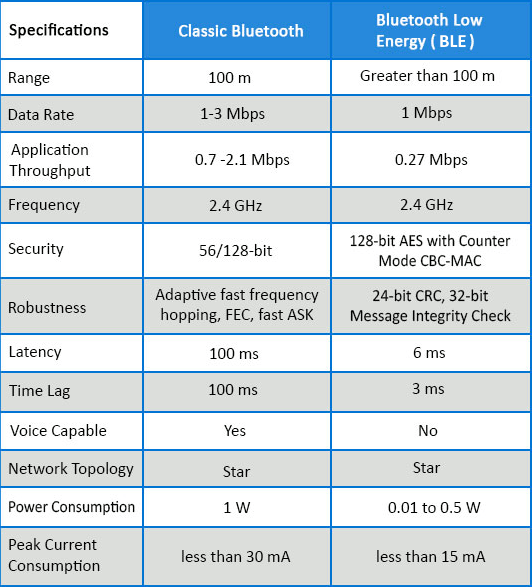
\includegraphics[scale=0.6]{imgs/blevsbt}
	\caption{Razlike između klasične Bluetooth i BLE tehnologije \cite{blevsbt}}
	\label{fig:blevsbt}
\end{figure}

Jedna od mana modula ESP32-C3 jest što ne podržava klasični Bluetooth. Iako BLE nudi prednosti u odnosu na \textit{BT Classic}, poput niske potrošnje i raznovrsnije podržane topologije, uređaji s BLE protokolom i s klasičnom Bluetooth tehnologijom ne mogu međusobno povezati. Ta činjenica ograničava povezivanje i korištenje ESP32-C3 modula, stoga ne može komunicirati s uređajima koji rade na temelju klasičnog Bluetootha. Većina audio uređaja, poput Bluetooth zvučnika, zbog potrebe za prijenosom velike količine podataka koriste klasični Bluetooth radi performansi. ESP32-C3 ne može se povezati s takvim uređajima.



\eject